\documentclass[tikz,border=10pt]{standalone}
\usepackage{tikz}
\begin{document}

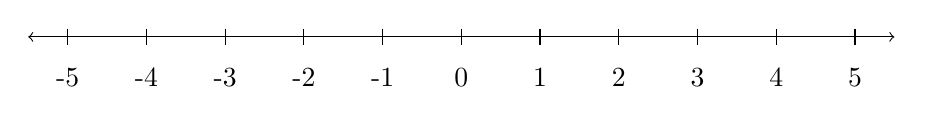
\begin{tikzpicture}
  % Draw the number line
  \draw[<->] (-5.5,0) -- (5.5,0) node[right] {};

  % Tick marks and labels
  \foreach \x in {-5,-4,-3,-2,-1,0,1,2,3,4,5}
    \draw[shift={(\x,0)},color=black] (0pt,3pt) -- (0pt,-3pt) node[below=5pt] {\x};

\end{tikzpicture}

\end{document}
